The formal design of algorithmic assurances is still an emerging field. Consequently, there are many opportunities for further research along different lines. This section outlines some possible promising directions for future work.

\subsection{Properties of Assurances} \label{sec:assurance_props_future}
 Figure~\ref{fig:refined_trust} gives some hints about how designers might be able to fully characterize the properties of AIA assurances. In this survey we investigate, in some detail, `Level of Integration'. However all of the other grayed-out boxes in Figure~\ref{fig:refined_trust} have open questions that should still be investigated. 

\subsubsection{Source-Target Classification}
    It is convenient to refer to assurances by way of their source and target. Intuitively, there may be a set of different algorithms that are useful for making assurances that convey information about planning to the competence dimension of the user's trust. It is easier to refer to these assurances in terms of their source and target. So, for this example that class of algorithms would be the `planning-competence' class.
    
    Not only is this useful shorthand for communicating about the purpose of the algorithms, but it is useful in classifying the range of assurance algorithms that exist. There may also be a class of algorithms that span multiple source-target capabilities. For example there may be a kind of algorithm that can give a `learning-competence' assurance, as well as a `planning-competence' assurance.

    This is especially true since many of the AIA capabilities can overlap. Also, the effects of assurances cannot be guaranteed to affect only one trust dimension.

    Figure \ref{fig:Assurance_classes} shows the hierarchy of proposed assurance classes. The categories mirror those of the trust model proposed by \citet{McKnight2001-fa}, but with the emphasis on what an AIA has the ability to most readily influence (and consequently where most research is found). The boxes with the beveled corner identify and define the different classes of assurances. All classes are included here for completeness and generality. Although, while it is hypothetically possible for an AIA to influence a persons general `Trusting stance' given enough time\footnote{One might imagine an AIA that specifically speaks to the human about the benefits or drawbacks about trusting even though there might not be evidence to do so, similar to the role a counselor might play}, the gray boxes are not considered further in this survey, as practically no direct research exists in the realm of human-AIA relationships.

    \textbf{ugggg, this gets a little complicated, but it's not supposed to be}.


\subsection{Component and Composite Assurances}
Assurances can be either component or composite. This was seen a little through the survey. The definitions are as follows:

\begin{description}
    \item [Component:] An assurance that originates from a single AIA capability source, and targets a single trust dimension target.
    \item [Composite:] The combination of more than one component assurance into a single assurance. 
\end{description}

\begin{figure}[!htbp]
    \centering
    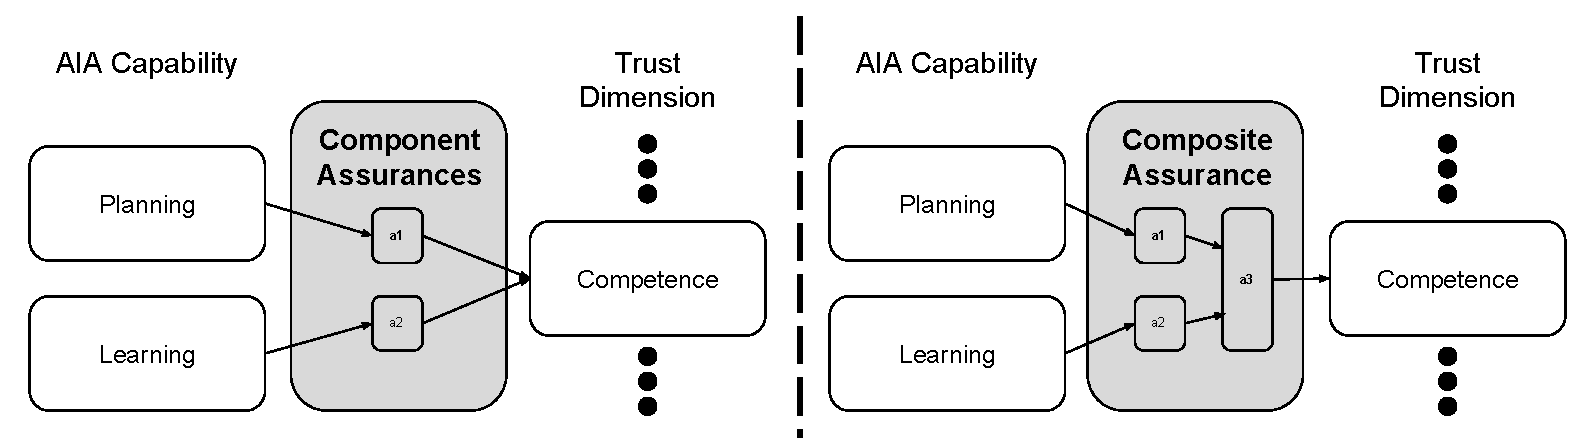
\includegraphics[width=0.9\textwidth]{Figures/Assurance_component_composite.pdf}
    \caption{Figure illustrating the difference between component and composite assurances. The existence of multiple assurances does not imply a composite assurances, rather the combination of multiple component assurances into a single assurance constitutes a composite assurance.}
    \label{fig:assurance_mapping}
\end{figure}

Figure \ref{fig:assurance_mapping} illustrates the concepts of component and composite assurances.

\paragraph{Component Assurances:} Component assurances are perhaps the most well researched in the existing literature. This is likely because several verified component assurances are the predecessors to composite ones. A component assurance might include displaying the confidence of a classification prediction, or visualizing a model as discussed in section \ref{sec:q2}.

\paragraph{Composite Assurances:} Composite assurances are assurances that are built of several components. A notable example is the work by \citet{Aitken2016-cv} who propose a measurement called `self-confidence', applicable to Partially Observable Markov Decision Processes (POMDPs). This metric combines five component assurances into a single composite assurance that is meant to distill the information into a value that a novice operator could understand easily. This paper was discussed in more detail in \ref{sec:q2}. 


\subsubsection{Explicit and Implicit Assurances}
\citet{Sheridan1984-kx} briefly alluded to the existence of explicit and implicit assurances when they discussed the nature of how humans behave when working with automated systems. They suggested that the operator's perception of the automated system can be effected by `performance' and its `reports on its own performance'. 


\begin{description}
    \item [Explicit:] Assurances that are purposefully given to affect the trust of a user.
    \begin{itemize}
        \item Legible motion \cite{Dragan2013-wd}, which is motion calculated with the intent of being more understandable by a human
        \item $R^2$ value, gives some indication of how well the regression accounts for the variance of the data
    \end{itemize}
    \item [Implicit:] All other assurances that aren't explicit.
    \begin{itemize}
        \item Reliability in completing a task. Generally, the object of success is not to affect the user's trust (although this is a nice side-effect).
        \item The way an autonomous vehicle appears. For example something that looks neat will have a different effect on trust, than an AIA with wires dragging on the ground. 
    \end{itemize}
\end{description}




\emph{Tutoring vs Telling:}
Most assurances investigated to date are `telling', in that they do not consider the experience or other traits of different users. The ability to adapt to different users, and to tutor them to appropriate trust will become more critical as time passes due to the diversity of users bases for advanced AIAs and time that users will interact with them. A tutoring assurance would be a planned, dynamic, sequence of assurances that would change in time to adapt to the user's needs. This might include modification of assurances to help a user avoid boredom, or to use the system differently in varying circumstances. It isn't surprising that, to our knowledge, no research has been done with respect to tutoring a user in a trust relationship. This is a complex problem to address that would involve understanding how different users learn, and what an appropriate strategy would be to teach them to have appropriate TRBs. However, a rich resource (not investigated in this paper) would be the work on tutoring systems \citet{Wenger2014-ld} and algorithmic teaching \citet{Balbach2009-jw}.


\subsection{Trust and Distrust}
The treatment of assurances in this survey is based, in part, on a model of interpersonal trust. For completeness it will be important to further investigate \textit{distrust}, as reviewed and discussed by \citet{Lewicki1998-ox}, and formalized in \citet{McKnight2001-gz}. Low trust is not the same as distrust, and low distrust is not the same as trust. \citet{McKnight2001-gz} suggest that `the emotional intensity of distrust distinguishes it from trust', and they explain that distrust comes from emotions like wariness, caution, and fear -- whereas trust stems from emotions like hope, safety, and confidence. Trust and distrust are orthogonal elements that define a person's TRB towards a trustee. Since distrust was not considered here, it is not clear to what extent the human-AIA trust model remains effective in the presence of user wariness, caution, or fear. Questions for future work include: to what extent can behaviors driven by distrust be isolated from those originating from trust? How can those behaviors be detected to begin with? And in what circumstances is the extra effort necessary? 

\subsection{Human Limitations}
Dealing with human users requires consideration of their cognitive limitations. For instance cognitive biases known as `framing effects' (reacting to the same choice in different ways depending on how it is presented) will be important to consider for designing usable AIAs that must make decisions under uncertainty ~\cite{Freedy2007-sg,Riley1996-qm}. While framing effects are not surprising to those familiar with cognitive science, they will likely be unanticipated phenomena to many AIA system designers. Other related cognitive biases and limitations such as `recency effects' (being biased in making choices based on recent experience), `focusing effects' (being biased in choice selection based on a single aspect of a correlated event), or `normalcy biases' (failure to consider situations which have never occurred before) are also important to consider. 

Besides cognitive biases, humans are also limited in their ability to understand certain kinds of information. Communities that investigate how probabilistic and statistical explanations can be presented to humans will have many insights that are relevant for AIA designers and assurance design \cite{Rouse1986-dz,Wallace2001-fm,Kuhn1997-qc,Lomas2012-ie,Swartout1983-ko}. But it is not immediately clear what methods are most appropriate for application in assurance design, or how they might be applied. For instance, can the AIA detect when cognitive limitations are effecting TRBs? What other user limitations need to be characterized? 

\subsection{Expression and Perception of Assurances} \label{sec:express_assurances}
Although specific algorithms can be used to build the contents of assurances, it is also critical to consider the actual communication of assurances. The expression (and subsequent perception) of an assurance involves considering mediums, methods, and efficacy. The medium of an assurance includes the form in which it expressed, e.g. visually, audibly, or otherwise. 
The method of expression includes for example using a plot, or a natural language phrase (which could be text-based or speech-based, depending on the medium).  Finally, the factors influencing the efficacy of the assurance must also be considered (e.g. consider using an audible assurance in a noisy environment). Humans generally utilize different methods/mediums when communicating assurances to each other to maintain efficacy when potential `losses in transfer' might occur. 
However, arguably the greatest challenge in using different mediums and methods is not in their implementation, but in designing the ability to recognize and decide when they should be applied. Some interesting questions are: In what circumstances are different methods most useful? And the same for mediums? How can different methods/mediums be selected in order to maximize assurance efficacy while also taking into account that using all possible combinations will \emph{not} help the user? How, and to what extent, can AIAs assess the efficacy of an assurance before, during, or after operation?

\subsection{Observing Effects of Assurances} \label{sec:measuring_effects}
    Since assurances are meant to influence TRBs, it is important to quantify those effects so that:  1) the AIA system designer can understand how effective the assurances are; and 2) the AIA can observe and respond to/adjust the efficacy of its assurances. To our knowledge, there has not been any work that enables an AIA to observe user responses to assurances and then adapt behaviors appropriately (at least not in the trust cycle setting). 
    Yet, this capability is crucial for enabling AIAs to meet different user's needs. 
Theoretically, any method that is made for the designer to measure the effects of assurances could also be deployed by the AIA itself to assess the effects of assurances on user TRBs. 
The surveyed literature gives some insights into how that has been done to date; namely, there are two main approaches: (1)  Gather self-reported changes in trust from human users; and (2) Measure changes in user's TRBs. 
    
\subsubsection{Self-Reported Changes in Trust} Assessing self-reported changes in trust involves asking users to answer questions, such as `how trustworthy do you feel the system is?'; or `to what extent do you find the system to be interpretable?', either while using a system or afterwards \cite{Mcknight2011-gv,Muir1996-gt,Wickens1999-la,Salem2015-md,Kaniarasu2013-ho}. These kinds of questions are useful in verifying whether the assurances are having the expected effects. It is not unreasonable to imagine that an AIA might be equipped to ask users questions about their trust, process those responses, and modify assurances appropriately.

Self-reports are the most useful when trying to understand the true effects of an assurance. Does a certain assurance, assumed to affect `situational normality', actually do that? 
Does displaying a specific plot actually convey information about `predictability'? 
There is much room for research in this area, which can be used to inform the selection of the methods of assurance. 
However, changes in self-reported trust do not always result in changes in TRBs \cite{Dzindolet2003-ts}. From the AIAs perspective this means that --- unless the object of the assurances is to make the person's level of self-reported trust change --- the assurances may not be providing any tangible benefit. 
As previously discussed, a more concrete objective for designing assurances in human-AIA interaction is to elicit appropriate TRBs from the human user. 
From this perspective, measuring changes in TRBs is the more direct and objective approach to assessing effectiveness.% of assurances.

\subsubsection{Measuring Changes in TRBs} Researchers often measure how long AIAs are able to run under full autonomy, before the autonomy is turned off by users \cite{Freedy2007-sg,Desai2012-rc}. 
Other researchers assess user's willingness to cooperate with AIAs \cite{Salem2015-md,Wu2016-ei,Bainbridge2011-pl}. 
A more ideal metric is the likelihood that users will use certain AIA capabilities `appropriately'. 
However, this is more difficult to formally define/calculate in different situations. 
As a concrete example for the UGV road network problem, %%%there is not an option to `turn off' the UGV's autonomy --but the user could switch off the planning feature...
the remote supervisor can make decisions such as accepting a plan or policy formulated by the UGV, or switching off the autonomous planner to provide their own plan to be implemented by the UGV. 
In this situation, the effect of assurances might be measured by how likely the operator is to accept a generated plan, instead of overriding it (recall that the goal may not be to have the generated plan accepted 100\% of the time, but rather that it be accepted with respect to how appropriate it is in a given context).

In practical application, assurances designed to lead the user to believe that the AIA is more competent, predictable or reliable than the user initially believed do not achieve their objectives if the user doesn't treat the AIA any differently than before/without the assurances. 
This assumes that it is possible for appropriate TRBs to be defined and observable in the first place. 
If, for example, an appropriate TRB hypothetically involves user verification of a sensor reading, can the AIA perceive whether or not such behavior takes place? 
%\edit{...good following: need to revise/polish...}
If the user is queried about this, can the user always be trusted to provide an honest/correct response or behave appropriately? 
%Is there a way to verify the user behavior is actually appropriate? 
This issue has gained notoriety with the current generation of autonomous cars, where users still need to attentively sit in the driver's seat in case the vehicle cannot perform correctly. This underscores the importance of designing methods for perceiving (in)appropriate TRBs. 
%
% \subsection{The Imprecise Nature of Assurances} \label{sec:imprecise_nature}
    % Due to the nature of trust (and humans in general), a single assurance might be targeted at influencing the competence dimension of trust, but it may also have effects on other dimensions. As an example an assurance that targets predictability may also have an affect on the probability of depending.
%
    % Besides being difficult to separate effects on a single user, individual users are different as well. Thus no assurance will have an identical effect when given to two separate users. This makes it difficult to have precise effects on user trust behaviors.
%
    % One might attempt to mitigate this uncertainty by using expressions that are more precise than others, such as displaying a probability distribution rather than on a maximum likelihood. This gets into some considerations about how the presentation of information affects the ability of a human to understand.

